
\begin{flushleft}
{\Large
\textbf{Supplementary Information 2 \\ Categorization of multinomial logistic regression \\}
}
\end{flushleft}

% Please keep the abstract below 300 words
%\section{Categorization of multinomial logistic regression using raw data and inferred features}
% Place figure captions after the first paragraph in which they are cited.
\begin{figure}[!h]
    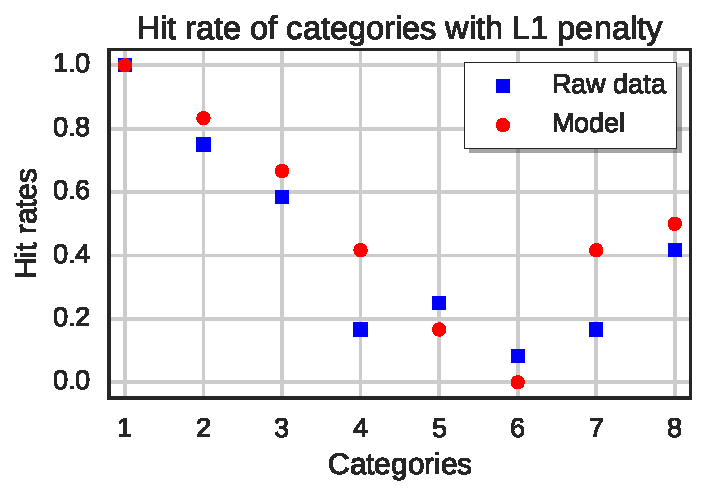
\includegraphics[width=.7\linewidth]{l1_hit_rate_2way}\\
    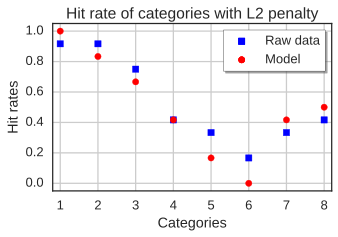
\includegraphics[width=.7\linewidth]{l2_hit_rate_2way}
	\caption{\bf Hit rates within eight categories} Compare the hit rates of actual data and inferred states of the macaque dataset. A. Multinomial logistic regression sing L1 regularization. Model inferred features outperform the raw data in 5/8 categories and tie in one category. Model wins. B. Multinomial logistic regression sing L2 regularization. Model inferred features outperform 3/8 categories and tie in one. Both tied.
	 %using raw data and inferred features for visual category dataset.
	\label{fig:softmax}
\end{figure}
